\documentclass[letterpaper,12pt]{article}
\usepackage{times}
\usepackage{helvet}
\usepackage{courier}
\usepackage{fancyheadings}
\pagestyle{fancy}
\usepackage{pmc}
\usepackage{graphicx}
\setlength\textwidth{6.5in}
\setlength\textheight{9.0in}
\begin{document}
\title{Eyes on the site\footnote{Henke's favorite line. See
  Figure~\ref{henke_screaming}}}
\author{ Ramesh Subramonian }
\maketitle
\thispagestyle{fancy}
\lfoot{{\small Data Analytics Team}}
\cfoot{}
\rfoot{{\small \thepage}}

Henke's favorite line is ``eyes on the site''. This paper discusses what
this means in terms of Data Products.

Derived data (or inferences) have three basic inputs
\begin{itemize}
\item user generated content
\item product requirements
\item algorithms
\end{itemize}
All three of these are constantly changing. I have listed them in
decreasing order of fluidity.

The nature of inferencing means that we will always be able to find
a few bad examples. There was a time when Googling for ``failure'' led
one to the White House. We cannot manage based on anecdotal experience. Hence,
the need for a Data Factory. The analogy to bear in mind is that 
``Ops is to Engineering as the Data Factory is to Data Analytics''.

The Data Factory is designed to enable operators to keep a finger on the
pulse of derived data. They need to be able to 
\begin{itemize}
\item ask the same question on different data sets --- sliced by geo,
  sliced by time, sliced by industry (Fortune 500 companies have
      different needs)
\item ask different questions on the same data set --- sliced by product
needs (ads versus search versus career explorer)
\end{itemize}

Empowering data operators requires
\begin{itemize}
\item powerful number-crunching algorithms at the back-end
\item simple, highly customized user interfaces on the front-end
\end{itemize}

Staffing against this need requires
\begin{itemize}
\item senior engineers with good quantitative skills, analytical
reasoning and an understanding of high performance and distributed
computing
\item junior engineers to cobble together user interfaces and write
automated tests for the system as a whole
\end{itemize}

The Data Factory is architected on a simple LAMP platform, designed to
have multiple ``mini-apps'' co-exist in a loosely coupled fashion. This
also allows us to farm out small, independent units of work.  
The request for an out-sourced junior engineer should be viewed in the
light of this framework --- both as an immediate need and a longer term
gamble that this architecture is the right one for the Data Factory.

\begin{figure}
\fbox{
  \begin{minipage}{18 cm}
  \centering
  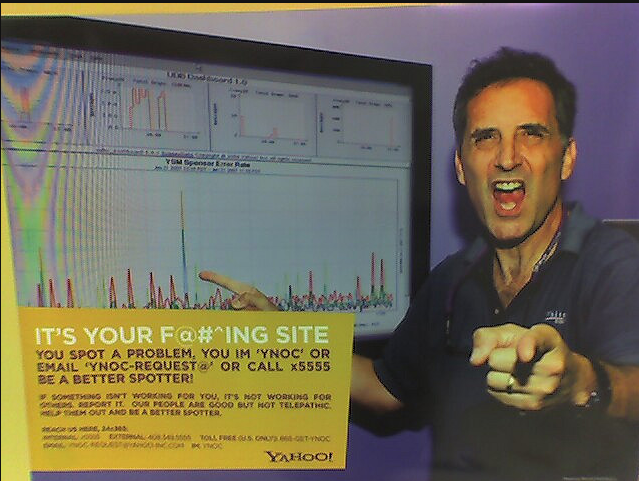
\includegraphics[width=6.5in]{henke_screaming.png}
  \caption{Henke's ``Eyes on the Site''}
  \label{henke_screaming}
  \end{minipage}
}
\end{figure}


\end{document}
